\begin{minted}[gobble=4,fontsize=\footnotesize]{tex}
    \section*{Введение}
    \addcontentsline{toc}{section}{Введение}
    Быстрое развитие промышленной автоматизации обусловило развитие методов и средств сбора данных и управления, начиная с всевозможных датчиков и заканчивая SCADA-системами. С развитием SCADA-систем возникла необходимость учёта и контроля многих узлов системы, не привязанных к измерительному оборудованию. Для обхода данного препятствия были задействованы беспроводные технологии: Wi-Fi, RFID, датчики определения местоположения объекта. В работе рассматривается внутренняя структура и алгоритм работы устройства определения расстояния между объектами методом \textit{Time of Flight}.

Радиолокация --- область науки и техники, объединяющая методы и средства локации (обнаружения и измерения координат) и определения свойств различных объектов с помощью радиоволн~\cite{wiki:radiolocation}.

Радиолокация позволяет использовать радиоволны для автоматизации различных целей и задач, в том числе --- автоматизации производств, АСУТП-систем и SCADA. Например, используя специальные <<радиометки>>, закрепляемые на движущихся объектах, можно отслеживать пути перемещения различного технологического оборудования, заготовок на складах и даже передвижение персонала.

В то время, как GPS, ГЛОНАСС и подобные системы позволяют отслеживать перемещение объекта на открытой местности, они не позволяют отслеживать его внутри помещений. Всвязи с этим, в современных условиях промышленной автоматизации стоит задача создания систем отслеживания местоположения всех критических объектов внутри цехов.

Простейшая задача радиолокации сводится к вычислению расстояний между тремя точками, а затем вычислению местоположения специализированными алгоритмами (например, методом триангуляции). Дипломная работа сфокусирована на определении расстояния между двумя точками методом \textit{Time of Flight}, а также расчётё погрешностей и задержек, возникающих во время измерения, и, как следствие, разрешающей возможности конечного устройства в зависимости от выбранного оборудования.


    \section{Электромагнитное излучение}

        \subsection{Физика радиоволн}
        Электромагнитная волна --- синусоидальное электромагтиное колебание в пространстве~\cite{meanders:radiovolny}. Другими словами, ЭМВ --- это направленный поток фотонов. Источником радиоволны может быть любой электрический проводник, в котором движется переменный электрический ток. Электромагнитная волна состоит из электрического и магнитного синусоидального колебания, ориентированных друг относительно друга перпендикулярно (рисунок~\ref{fig:emf}).

\begin{figure}[ht]
    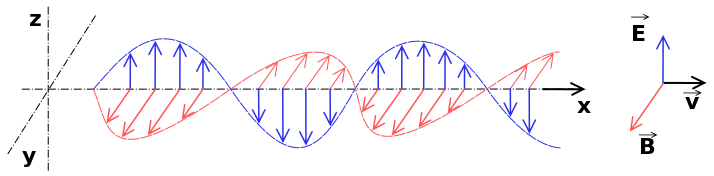
\includegraphics[width=.8\linewidth]{Figures/emf.png}
    \caption{Электромагнитная волна}
    \label{fig:emf}
\end{figure}

Радиоволны --- электромагнитное излучение с длинами волн в электромагнитном спектре длиннее инфракрасного света~\cite{wiki:radiowaves}. Радиоволны имеют частоту от 3 кГц до 300 ГГц, и соответствующую длину волны от 1 миллиметра до 100 километров. Естественными источниками радиоволн являются молнии и астрономические объекты. Искусственно созданные радиоволны используются для стационарной и мобильной радиосвязи, радиовещания, радиолокации и других навигационных систем, спутников связи, компьютерных сетей и других бесчисленных приложений. Различные частоты радиоволн по-разному распространяются в атмосфере Земли: длинные волны могут покрыть часть Земли очень последовательно, более короткие волны могут отражаться от ионосферы и распространяются по всему миру, и с еще более короткими длинами радиоволны изгибаются или отражаются очень слабо и распространяются в пределах прямой видимости.

Земная атмосфера прозрачна почти полностью для падающего извне излучения лишь в двух сравнительно узких окнах: оптическом --- в диапазоне длин волн $\lambda$ от 0.3 мкм до 2 мкм (область до 8 мкм состоит из ряда узких полос пропускания) и в радиодиапазоне --- для волн длиной от 1 мм до 30 м~\cite{astronet:atmosphere}. Непрозрачность атмосферы для всех др. длин волн определяется поглощением и рассеянием излучения на молекулах и атомах, а также отражением радиоволн от электронов ионосферы (рисунок~\ref{fig:atmosphere}~\cite{wiki:radiowaves}).

\begin{figure}[ht]
    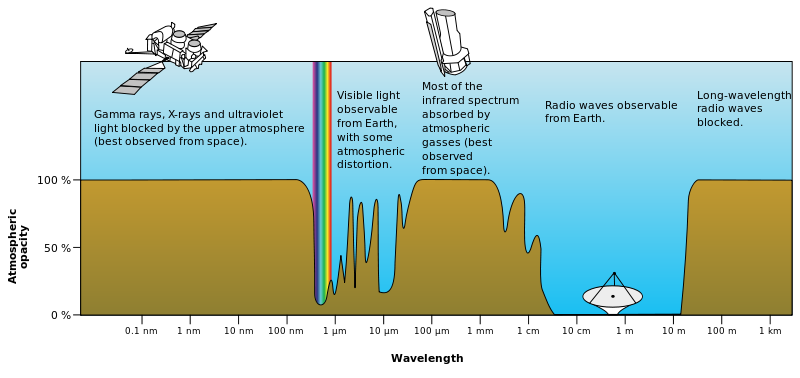
\includegraphics[width=1\linewidth]{Figures/radiowaves.png}
    \caption{Непрозначность атмосферы Земли для различных длин волн электромагнитного излучения, включая радиоволны}
    \label{fig:atmosphere}
\end{figure}

Электромагнитные волны (радиоволны) распространяются в вакууме со скоростью света --- 299, 792, 458 м/с.

Частота колебаний выражается через длину волны (формула~\eqref{eq:lambda}):

\begin{equation}
    \label{eq:lambda}
    f = \frac{c}{\lambda},
\end{equation}

где f --- частота, $\lambda$ --- длина волны, c --- скорость света.

Радиоволны подразделяются на несколько диапазонов (таблица~\ref{tab:radiorange}):

\begin{longtable}[c]{|c|c|c|}
    \caption{Диапазон радиоволн}
    \label{tab:radiorange}\\
    \hline
    \textbf{Диапазон} & \textbf{Частота} & \textbf{Длина волны}\\
    \hline
    \endfirsthead
    \hline
    \textbf{Диапазон} & \textbf{Частота} & \textbf{Длина волны}\\
    \hline
    \endhead
        Сверхдлинные <<СДВ>> & 3 -- 30 кГц & 100 -- 10 км\\
        \hline
        Длинные <<ДВ>> & 30 -- 300 кГц & 10 -- 1 км\\
        \hline
        Средние <<СВ>> & 300 -- 3000 кГц & 1000 -- 100 м\\
        \hline
        Короткие <<КВ>> & 3 -- 30 МГц & 100 -- 10 м\\
        \hline
        Ультракороткие <<УКВ>> & 30 МГц -- 6000 ГГц & 10 м -- 0.05 мм\\
        \hline
\end{longtable}

Ультракороткие, в свою очередь, включают (таблица~\ref{tab:ultrarange}):

\begin{longtable}[c]{|c|c|c|}
    \caption{Ультракороткие радиоволны}
    \label{tab:ultrarange}\\
    \hline
    \textbf{Диапазон} & \textbf{Частота} & \textbf{Длина волны}\\
    \hline
    \endfirsthead
    \hline
    \textbf{Диапазон} & \textbf{Частота} & \textbf{Длина волны}\\
    \hline
    \endhead
        Метровые <<МВ>> & 30 -- 300 МГц & 10 -- 1 м\\
        \hline
        Дециметровые <<ДМВ>> & 300 -- 3000 МГц & 10 -- 1 дм\\
        \hline
        Сантиметровые <<СМВ>> & 3 -- 30 ГГц & 10 -- 1 см\\
        \hline
        Миллиметровые <<ММВ>> & 30 -- 300 ГГц & 10 -- 1 мм\\
        \hline
        Субмиллиметровые <<СММВ>> & 300 -- 6000 ГГц & 1 -- 0.05 мм\\
        \hline
\end{longtable}

Диапазоны от дециметровых до миллиметровых волн, из-за их очень высокой частоты, называют сверхвысокими частотами <<СВЧ>>.

Распространение волны ограничивается её длиной: чем выше длина волны (меньше частота), тем она более способна огибать препятствия.


        \subsection{Передача информации радиоволнами}
        Для передачи информации радиоволну необходимо модулировать сигналом, содержащим информацию. Длинные, средние и короткие волны обычно имеют амплитудную модуляцию <<AM>>. Ультракороткие волны обычно имеют частотную модуляцию <<FM>>.

Модуляция (лат. modulatio --- размеренность, ритмичность) --- процесс изменения одного или нескольких параметров высокочастотного несущего колебания по закону низкочастотного информационного сигнала (сообщения)~\cite{wiki:modulation}.

Передаваемая информация заложена в управляющем (модулирующем) сигнале, а роль переносчика информации выполняет высокочастотное колебание, называемое несущим. Модуляция, таким образом, представляет собой процесс <<посадки>> информационного колебания на заведомо известную несущую.

В результате модуляции спектр низкочастотного управляющего сигнала переносится в область высоких частот. Это позволяет при организации вещания настроить функционирование всех приёмо-передающих устройств на разных частотах с тем, чтобы они <<не мешали>> друг другу.

Амплитудная модуляция представлена на рисунке~\ref{fig:am}. Этот тип модуляции изменяет \textbf{амплитуду} несущей частоты под действием кодирующего колебания (сигнала). Главный её недостаток --- низкая помехоустойчивость.

\begin{figure}[ht]
    \subfloat[]{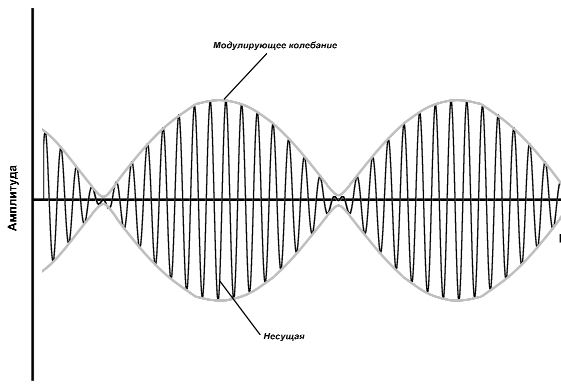
\includegraphics[width=.6\linewidth]{Figures/am.jpg}}
    \subfloat[]{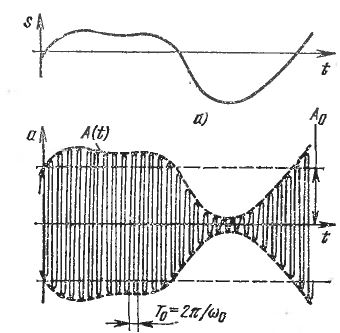
\includegraphics[width=.4\linewidth]{Figures/amclose.jpg}}
    \caption{Амплитудная модуляция (а) общая картина; (б) изменение несущего колебания по заданному закону}
    \label{fig:am}
\end{figure}

Частотная модуляция (рисунок~\ref{fig:fm}) --- изменение несущей \textbf{частоты} под воздействием кодирующего сигнала. Этот вид модуляции имеет более высокую помехоустойчивость несмотря на свою аналоговую природу.

\begin{figure}[ht]
    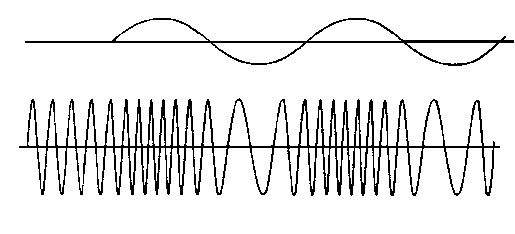
\includegraphics[width=.8\linewidth]{Figures/fm.jpg}
    \caption{Частотная модуляция}
    \label{fig:fm}
\end{figure}

Фазовая модуляция (рисунок~\ref{fig:pm}) --- изменение фазы несущей частоты скачкообразно (манипуляция). Недостаток данной модуляции в том, что ошибка в одном символе может привести к некорректному приёму всех последующих.

\begin{figure}[ht]
    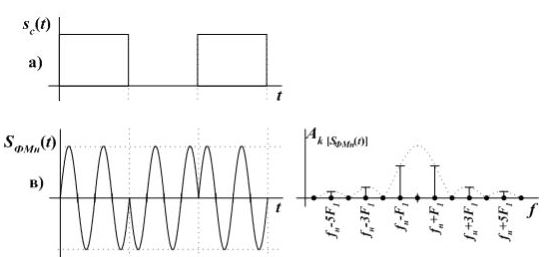
\includegraphics[width=.8\linewidth]{Figures/pm.jpg}
    \caption{Фазовая модуляция}
    \label{fig:pm}
\end{figure}

Дифференциально-фазовая манипуляция --- изменение фазы несущей частоты только при изменении разности (в данном случае --- при приходе каждой <<1>>).


        \subsection{Устройство радиопередатчика}
        Современный радиопередатчик состоит из следующих конструктивных частей (рисунок~\ref{fig:radiostruct})~\cite{wiki:radiotransmitter}:

\begin{itemize}
    \item задающий генератор частоты (фиксированной или перенастраиваемой) несущей волны;
    \item модулирующее устройство, изменяющее параметры излучаемой волны (амплитуду, частоту, фазу или несколько параметров одновременно) в соответствии с сигналом, который требуется передать (часто задающий генератор и модулятор выполняют в одном блоке — возбудитель);
    \item усилитель мощности, который увеличивает мощность сигнала возбудителя до требуемой за счёт внешнего источника энергии;
    \item устройство согласования, обеспечивающее максимально эффективную передачу мощности усилителя в антенну;
    \item антенна, обеспечивающая излучение сигнала.
\end{itemize}

\begin{figure}[ht]
    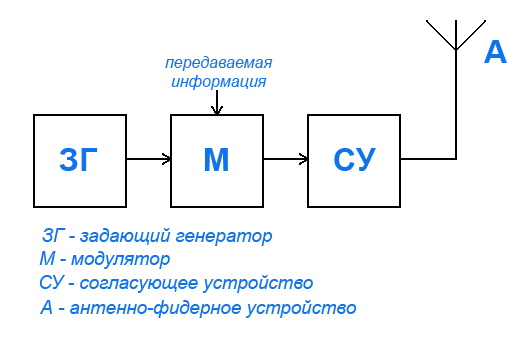
\includegraphics[width=.6\linewidth]{Figures/radiostruct.jpg}
    \caption{Структурная схема радиопередатчика}
    \label{fig:radiostruct}
\end{figure}

Принципиальная схема простейшего радиопередатчика представлена на рисунке~\ref{fig:rfcircuit}.

\begin{figure}[ht]
    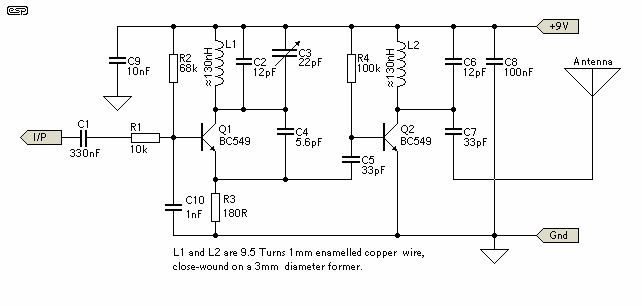
\includegraphics[width=1\linewidth]{Figures/rfcircuit.png}
    \caption{Простейшая принципиальная схема радиопередатчика}
    \label{fig:rfcircuit}
\end{figure}


        \subsection{Подбор правильной антенны}
        Антенна --- устройство, преобразующее энергию высокочастотного колебания от передатчика в электромагнитную волну, способную распространяться в пространстве. Или в случае приёма --- производит обратное преобразование (электромагнитную волну в ВЧ колебания)~\cite{habr:antenna}.

Простейшая антенна --- симметричный вибратор: два токопроводящих отрезка, каждый из которых равен 1/4 длины волны (рисунок~\ref{fig:symvibr}). Широко применяется для приема телевизионных передач, как самостоятельно, так и в составе комбинированных антенн. Так, к примеру, если диапазон метровых волн телепередач проходит через отметку 200 МГц, то длина волны будет равна 1,5 м. Каждый отрезок симметричного вибратора будет равен 0,375 метра.

\begin{figure}[ht]
    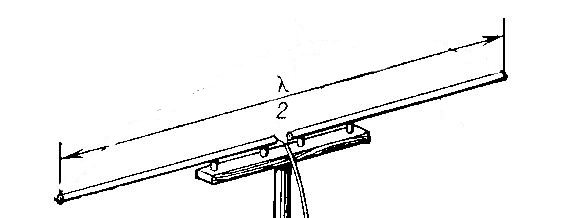
\includegraphics[width=.6\linewidth]{Figures/symvibr.jpg}
    \caption{Симметричный вибратор}
    \label{fig:symvibr}
\end{figure}

Несимметричный вибратор (штырьевая антенна) --- <<половина>> симметричного вибратора, установленного вертикально (рисунок~\ref{fig:asymvibr}). В качестве длины вибратора, применяют 1, 1/2 или 1/4 длины волны. Коэффициент направленного действия у несимметричного вибратора в два раза больше, чем у симметричного, за счет того, что вся мощность излучается в более узком направлении.

\begin{figure}[ht]
    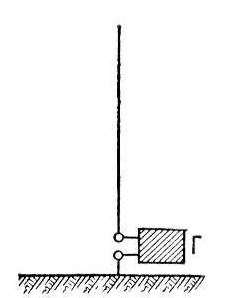
\includegraphics[width=.2\linewidth]{Figures/asymvibr.jpg}
    \caption{Несимметричный вибратор}
    \label{fig:asymvibr}
\end{figure}

При использовании приёмопередатчиков, работающих на частоте 433 МГц, длина волны $\lambda = 692$ мм. Соответственно, длина штырьевой антенны будет равна 69.2, 34.6 или 17.3 см.

Также существуют другие, более сложные типы антенн.

Поляризация --- это направленность вектора электрической составляющей электромагнитной волны в пространстве. Различают: вертикальную, горизонтальную и круговую поляризацию (рисунок~\ref{fig:polarization}).

\begin{figure}[ht]
    \subfloat[]{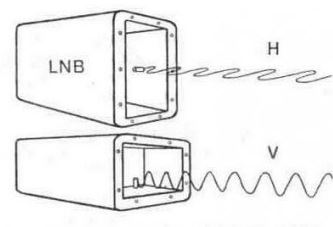
\includegraphics[width=.5\linewidth]{Figures/vgpolar.jpg}}
    \subfloat[]{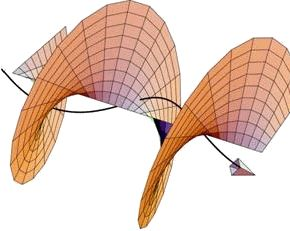
\includegraphics[width=.5\linewidth]{Figures/circlepolar.jpg}}
    \caption{Поляризация (а) горизонтальная и вертикальная; (б) круговая}
    \label{fig:polarization}
\end{figure}

Поляризация зависит от типа антенны и её расположения. К примеру, вертикально расположенный несимметричный вибратор, дает вертикальную поляризацию, а горизонтально расположенный --- горизонтальную.

Антенны горизонтальной поляризации дают больший эффект, т. к. природные и индустриальные помехи, имеют в основном вертикальную поляризацию. Горизонтально поляризованные волны, отражаются от препятствий менее интенсивно, чем вертикально. При распространении вертикально поляризованных волн, земная поверхность поглощает на 25\% меньше их энергии.


    \section{Принципы радиолокации}
    Радиолокацией называется обнаружение, определение координат и параметров движения различных объектов (целей), отражающих, переизлучающих или излучающих электромагнитную энергию (радиоволны). Термин <<локация>> происходит от латинского location – размещение, расположение. Комплекс радиотехнических устройств, выполняющих указанную задачу, представляет собой радиолокационную станцию (РЛС), или радиолокатор.

Радиолокация основана на следующих физических явлениях~\cite{wiki:radiolocation}:

\begin{enumerate}
    \item Радиоволны рассеиваются на встретившихся на пути их распространения электрических неоднородностях (объектами с другими электрическими свойствами, отличными от свойств среды распространения). При этом отражённая волна, также, как и собственно, излучение цели, позволяет обнаружить цель.
    \item На больших расстояниях от источника излучения можно считать, что радиоволны распространяются прямолинейно и с постоянной скоростью, благодаря чему имеется возможность измерять дальность и угловые координаты цели (Отклонения от этих правил, справедливых только в первом приближении, изучает специальная отрасль радиотехники --- Распространение радиоволн. В радиолокации эти отклонения приводят к ошибкам измерения).
    \item Частота принятого сигнала отличается от частоты излучаемых колебаний при взаимном перемещении точек приёма и излучения (эффект Доплера), что позволяет измерять радиальные скорости движения цели относительно РЛС.
    \item Пассивная радиолокация использует излучение электромагнитных волн наблюдаемыми объектами, это может быть тепловое излучение, свойственное всем объектам, активное излучение, создаваемое техническими средствами объекта, или побочное излучение, создаваемое любыми объектами с работающими электрическими устройствами.
\end{enumerate}

Основа радиолокации --- нахождение прямолинейного расстояния между объектами. Например, если найти расстояние от одного и того же объекта к двум различным <<искателям>>, можно будет аналитически рассчитать угол и относительно точное местоположение объекта.


    \section{Реализация метода ToF}

        \subsection{Принцип метода ToF}
        Реализация метода \textit{Time of Flight} заключается в следующем: радиоволна летит от источника к приёмнику, который работает в режиме ретранслятора. Приёмник отправляет сигнал назад источнику, который фиксирует время полёта сигнала. Поделив это время на 2, получим время полёта сигнала от источника к приёмнику (формула~\eqref{eq:timeflight}):

\begin{equation}
    \label{eq:timeflight}
    t = \frac{T_f}{2},
\end{equation}

где $T_f$ --- время полёта (flight) от источника к приёмнику и обратно.

На рисунке~\ref{fig:tofscheme} представлена функциональная схема такого устройства.

\begin{figure}[ht]
    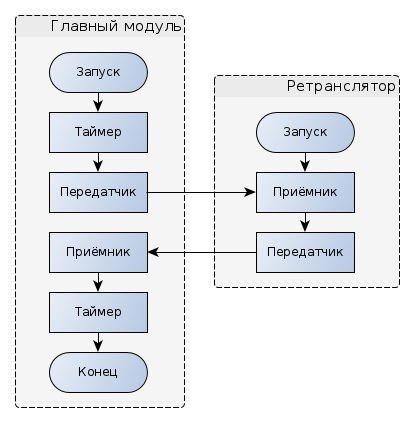
\includegraphics[width=.65\linewidth]{Figures/tofscheme.png}
    \caption{Функциональная схема устройства \textit{Time of Flight}}
    \label{fig:tofscheme}
\end{figure}

Электромагнитное излучение преодолевает расстояние со скоростью около 300.000.000 м/с. Таким образом, чтобы успеть <<словить>> время пролёта электромагнитной волны, детектор должен работать на частоте, равной или превышающей время пролёта сигнала от источника к приёмнику и обратно (формула~\eqref{eq:freqflight}). Чем более высокой будет частота работы устройства, тем больше будет его разрешающая способность и тем более точные результаты мы получим.

\begin{equation}
    \label{eq:freqflight}
    f = \frac{1}{T_f} = \frac{c}{S},
\end{equation}

где c --- скорость света, S --- минимально возможное расстояние, на котором прибор с данной частотой должен успевать уловить время $T_f$ полёта радиоволны.

Таким образом, для обеспечения работы на расстоянии в 3 метра, устройство должно работать на частоте как минимум $f = \frac{300.000.000}{3} = 100$ МГц. Для 300 метров --- 1 МГц.

Для уменьшения необходимой частоты работы устройства, а также сокращению возможных погрешностей и ошибок, воспользуемся методом <<накопления>> ToF.


        \subsection{Принцип метода <<накопления>> ToF}
        \label{sec:accumulation}
        Метод <<накопления>> ToF заключается в следующем: устройство с заведомо более низкой частотой, чем необходимо, неспособное уловить время $T_f$ на заданном расстоянии, производит ту же последовательность действий (посылает сигнал ретранслятору и принимает его назад), но не останавливается, а продолжает посылать и принимать сигнал N-ное количество раз. Через заданный интервал времени (или через заданное число N итераций) устройство останавливается и определяет <<накопленное>> суммарное <<добавочное>> время. Это время, с определённой погрешностью, и будет временем $T_f \cdot N$ полёта, умноженным на N (рисунок~\ref{fig:accscheme}).

\begin{figure}[ht]
    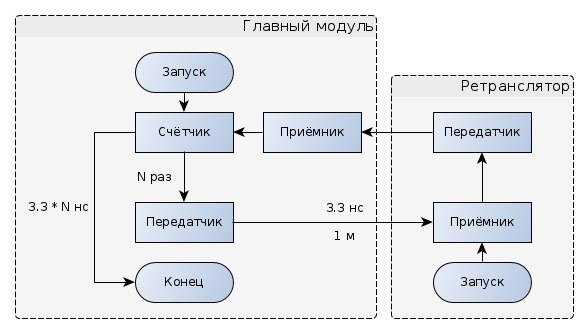
\includegraphics[width=1\linewidth]{Figures/accscheme.png}
    \caption{Функциональная схема метода <<накопления>> ToF}
    \label{fig:accscheme}
\end{figure}

Однако у данного метода есть и недостатки: чем ниже частота, тем больше будет время накопления результата. Для примера, возьмём частоту 1 Гц и расстояние 1 м. Тогда передатчик будет посылать данные приёмнику, ждать возврата сообщения, затем ждать секунду и посылать очередной пакет приёмнику.

На расстоянии 1 м. время полёта пакета от источника к приёмнику будет равно $T_f = \frac{1}{300.000.000} = 3.3$ нс.

Как будет сказано ниже, разрешение (погрешность) микроконтроллеров ATmega (Arduino) составляет около 4-10 мксек. В данном примере, возьмём 50 мксек для надёжности. Время, необходимое для того, чтобы микроконтроллер зарегистрировал изменение, будет равно:

\begin{equation}
t_w = \frac{\Delta\tau}{T_f} = \frac{50 \cdot 10^{-6}~\textrm{с}}{3.3 \cdot 10^{-9}~\textrm{с}} = 15151~\textrm{с} = 252~\textrm{мин} = 4.2~\textrm{ч}
\end{equation}

Обычно на практике применяются расстояния больше 1 метра, что сокращает время ожидания результата пропорционально расстоянию. Задача сводится к увеличению частоты работы устройства.


        \subsection{Расчёт ошибок измерений расстояния методом ToF}
        Нижнюю границу диапазона ошибки TOF-метода абстрактно можно вычислить, используя вариант неравенства Крамера-Рао~\cite{radiofreq:tof}, представленный в формуле~\eqref{eq:cramer} (рисунок~\ref{fig:cramer}):

\begin{equation}
    \label{eq:cramer}
    \sigma^2_{TOF} >= \frac{1}{8\pi^2 \cdot \beta^2_f \cdot SNR \cdot n},
\end{equation}

где $\sigma^2_{TOF}$ --- дисперсия (ошибка TOF), $\beta_f$ --- спектральная ширина полученного сигнала в герцах, n --- число усреднённых TOF-измерений, SNR --- энергия на бит делённая на мощность шума ($E_b/N_0$).

\begin{figure}[ht]
    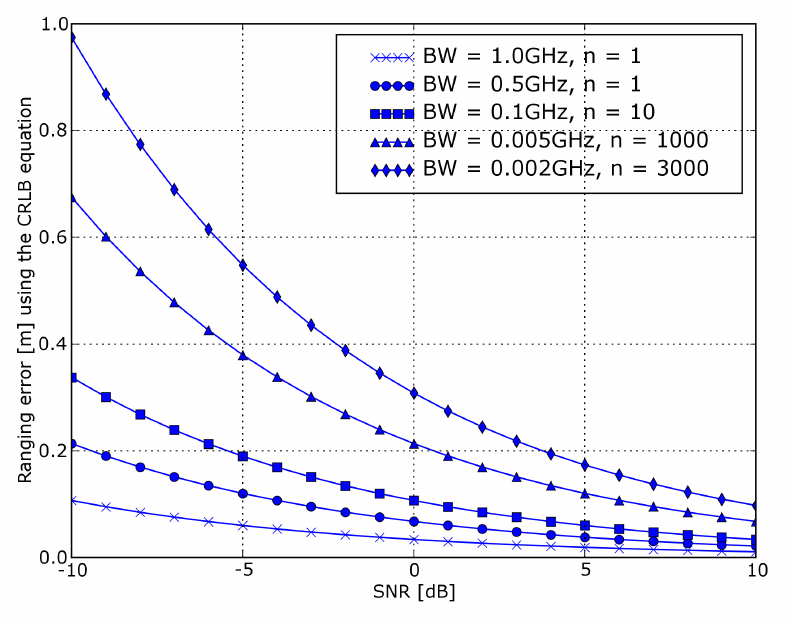
\includegraphics[width=.7\linewidth]{Figures/cramer.png}
    \caption{Нижняя граница диапазона TOF-ошибки}
    \label{fig:cramer}
\end{figure}

Из формулы~\eqref{eq:cramer} видно, что точность TOF-измерения квадратично растёт с увеличением спектральной ширины сигнала, из чего следует эффективность использования сверхширокой полосы. Всвязи с этим, делается вывод о невыгодности использования свободных 433-МГц несущих частот для передачи радиосигнала.


        %ABSTRACT MAIN part

    \section{Микроконтроллеры}
    \label{sec:microcontroller}
    Микроконтроллер (англ. \textit{Micro Controller Unit, MCU}) --- микросхема, предназначенная для управления электронными устройствами \cite{wiki:microcontroller}. Типичный микроконтроллер сочетает на одном кристалле функции процессора и периферийных устройств, содержит ОЗУ и (или) ПЗУ. По сути, это однокристальный компьютер, способный выполнять относительно простые задачи. Микроконтроллер общается с внешним миром считывая значения на своих <<входах>> и выдавая соответствующие значения на своих <<выходах>>.

Общая структурная схема микроконтроллера представлена на рисунке~\ref{fig:microstruct}.

\begin{figure}[ht]
    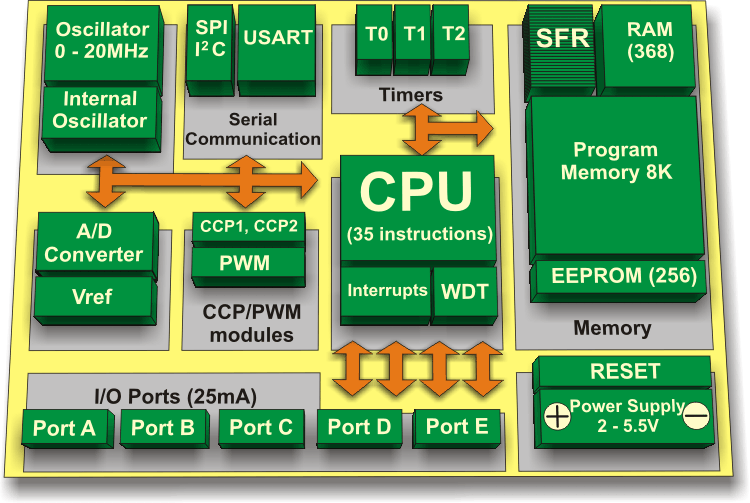
\includegraphics[width=.7\linewidth]{Figures/microstruct.png}
    \caption{Обобщённая структурная схема микроконтроллера}
    \label{fig:microstruct}
\end{figure}

Здесь можно наблюдать:

\begin{itemize}
    \item генератор задающей частоты (clock);
    \item последовательный UART-порт коммуникации с другими устройствами (например, по протоколу modbus);
    \item низкоуровневые таймеры (работающие на частотах начиная от задающей частоты и ниже);
    \item процессор с поддержкой прерываний;
    \item модуль широтно-импульсной модуляции;
    \item ЦАП/АЦП;
    \item порты ввода-вывода (аналоговые и цифровые);
    \item блок оперативной (RAM) и постоянной (EEPROM) запоминающей памяти.
\end{itemize}

Зачастую, частота работы микроконтроллеров недостаточна для обеспечения необходимой разрешающей способности Time of Flight устройства, и прибегают к \textbf{микропроцессорным} средствам, например платам на ARM-процессорах. Однако для целей моделирования был взят микроконтроллер ATMega, а точнее --- плата разработки Arduino, использующая в своём ядре микроконтроллер ATMega.


        \subsection{Характеристики и устройство ATmega (328)}
        Фирма ATMEL --- один из лидеров производства микроконтроллеров. Микроконтроллеры ATmega в большинстве своём работают на частоте 16 МГц. Это означает, что одна инструкция программы выполняется за 1/16000000 секунды, т. е. выполняется 16 миллионов инструкций за 1 секунду. Блок-схема ATmega328 показана на рисунке~\ref{fig:atmegablock}~\cite{atmega:328}.

\begin{figure}[ht]
    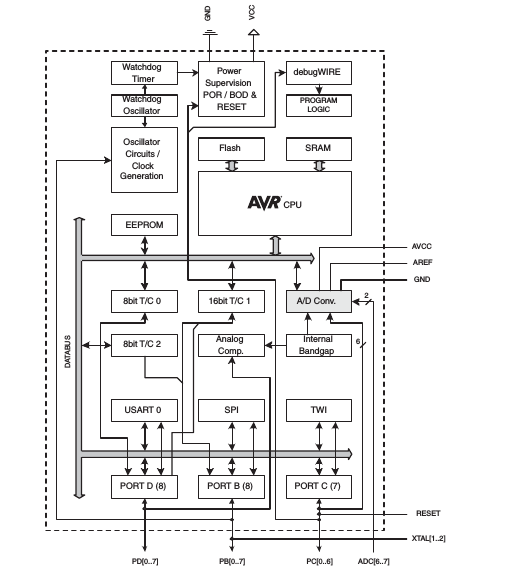
\includegraphics[width=.6\linewidth]{Figures/atmegablock.png}
    \caption{Блок-схема ATmega328}
    \label{fig:atmegablock}
\end{figure}


        \subsection{Аппаратно-программная среда Arduino}
        Arduino --- аппаратно-программная платформа <<надстройки>> над микроконтроллерами ATmega, позволяющая быстро и удобно конструировать прототип устройства без необходимости подавать внешнее питание и позволяющая разрабатывать безпаечные макеты.

Arduino представляет собой плату, построенную вокруг ATmega, поддерживающую высокоуровневые инструкции на языке C++, а также предоставляющую удобный интерфейс для программирования через USB-интерфейс. Благодаря большому сообществу и наличию разных библиотек, разработка конечныйх устройств на Arduino представляет собой удобный и быстрый процесс по сравнению с работой непосредственно с микроконтроллером.

Схематика Arduino UNO представлена в приложении A.

Технические характеристики Arduino UNO и Arduino MEGA представлены в таблице~\ref{tab:megatech}~\cite{arduino:mega, arduino:uno}.

\begin{longtable}[c]{|p{2in}|c|c|}
    \caption{Технические характеристики Arduino UNO и Arduino MEGA}
    \label{tab:megatech}\\
    \hline
    \textbf{Параметр} & \textbf{UNO} & \textbf{MEGA}\\
    \hline
    \endfirsthead
    \hline
    \textbf{Параметр} & \textbf{UNO} & \textbf{MEGA}\\
    \hline
    \endhead
        Микроконтроллер & ATmega328 & ATmega2560\\
        \hline
        Оперируемое напряжение & \multicolumn{2}{c|}{5 В}\\
        \hline
        Входное напряжение (реккомендуемое) & \multicolumn{2}{c|}{7 -- 12 В}\\
        \hline
        Входное напряжение (максимальное) & \multicolumn{2}{c|}{6 -- 20 В}\\
        \hline
        Цифровые входы/выходы & 14 (~6) & 54 (~14)\\
        \hline
        Аналоговые входы & 6 & 16\\
        \hline
        Постоянные ток на 1 вход/выход & \multicolumn{2}{c|}{40 мА}\\
        \hline
        Постоянный ток на вход 3.3 В & \multicolumn{2}{c|}{50 мА}\\
        \hline
        Память & 32 Кб & 256 Кб\\
        \hline
        Частота задающего генератора & \multicolumn{2}{c|}{16 МГц}\\
        \hline
\end{longtable}

Условные обозначения элементов на плате Arduino показаны на рисунке~\ref{fig:specuno}.

\begin{figure}[ht]
    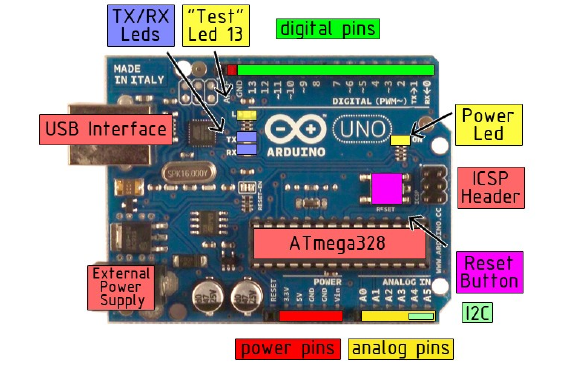
\includegraphics[width=.8\linewidth]{Figures/specuno.png}
    \caption{Спецификация Arduino UNO}
    \label{fig:specuno}
\end{figure}


    \section{Расчёт необходимой частоты и определение максимальной частоты оборудования}
    Метод \textit{Time of Flight} заключается в измерении времени полёта электромагнитной волны от источника к приёмнику и обратно. На основе этого осуществляется расчёт расстояния между двумя точками. \textit{Time of Flight} применяется внутри помещений с большим количеством <<радиометок>>, где необходима большая точность. Однако, с точностью растут и необходимые требования к конечному устройству.

Всвязи с этим, ставятся следующие задачи:

\begin{itemize}
    \item устройство должно работать на относительно высокой стабильной частоте: для точности измерения в 1 метр частота работы должна быть 300 МГц;
    \item необходима точная синхронизация времени: расхождение начального отсчёта времени источника и приёмника значительно скажется на результате измерения;
    \item мельчайшие шумы будут сказываться на результате, уменьшая точность измерения;
    \item необходимо учитывать всевозможные задержки оборудования, а также возможные отклонения генераторов тактовой частоты друг от друга, т. к. \textit{Time of Flight} очень чувствителен к погрешностям: маленькие отклонения времени дают большие отклонения расстояния;
    \item необходимо разработать быстрый и стабильный протокол общения передатчика и приёмника друг с другом.
\end{itemize}

В конечном итоге, необходимо выбрать оборудование с минимальными задержками, вычислить постоянную аппаратную задержку и описать программную модель измерения расстояния методом \textit{Time of Flight}.

Для устранение ошибки рассинхронизации <<часов>> приёмника и источника применяют метод \textit{TWTT (Two-way time transfer)}. Этот метод снижения ошибки измерения подробно описан в главе~\ref{sec:mitigation} <<\nameref{sec:mitigation}>>.

В работе рассматривается возможность построения <<Time of Flight>> устройства на микроконтроллерной базе, а также все препятствия на пути реализации такого устройства и погрешности измерений.


        \subsection{Определение максимальной частоты Arduino}
        Для определения максимальной скорости работы микроконтроллера, напишем программу, которая будет выдавать на одном из выходов контроллера прямоугольный сигнал. Воспользуемся функцией \textit{arduino} \textbf{micros()}, которая возвращает время работы контроллера в микросекундах:

\begin{minted}[gobble=4,fontsize=\footnotesize]{c}
    unsigned long initial = 0; //0 - 4,294,967,295
    unsigned long final = 0;
    int i; //-32,768 - 32,767

    void setup(){
        Serial.begin(9600);
    }

    void loop(){
        initial = micros();
        for (i = 0; i < 1E4; i++){
            digitalWrite(13, HIGH); //Turn on LED 13
            digitalWrite(13, LOW);  //Turn off LED 13
        }
        final = micros();
        Serial.println(final - initial);
        while (final > 1E7); //Stop after 10 seconds
    }
\end{minted}

Здесь мы замеряем текущее количество прошедших микросекунд, затем устанавливаем значение напряжения на 13-ом контакте Arduino сначала вверх, потом вниз, и повторяем эти действия $1 \cdot 10^4$ раз, затем замеряем новое значение количества прошедших микросекунд и показываем пользователю разницу между новым и старым значением функции \textbf{micros()}. Таким образом, мы получим значение времени в микросекундах, за которое сигнал на 13-ом выходе Arduino изменит своё значение 10000 раз.

Получим следующий результат:

\begin{longtable}[c]{|c|c|}
    \caption{Результат digitalWrite}
    \label{digitalWriteResult}\\
    \hline
    \textbf{Количество, шт} & \textbf{Результат, мкс}\\
    \hline
    \endfirsthead
    \hline
    \textbf{Количество, шт} & \textbf{Результат, мкс}\\
    \hline
    \endhead
        1 & 145884\\
        \hline
        13 & 145920\\
        \hline
        18 & 145924\\
        \hline
        35 & 145928\\
        \hline
        2 & 145932\\
        \hline
\end{longtable}

\begin{figure}[ht]
    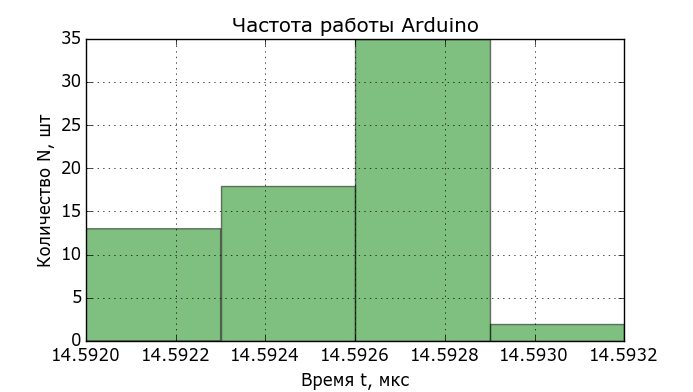
\includegraphics[width=.8\linewidth]{Figures/ardhist.png}
    \caption{Гистограмма измерений частоты Arduino}
    \label{fig:ardhist}
\end{figure}

Другими словами, дли включения и выключения одного выхода микроконтроллера \textbf{10000} раз нам понадобилось \textbf{145928} микросекунд, или \textbf{146} миллисекунд.

Одно включение и выключение выхода занимает $\frac{145928}{10000} = 14.5928$ микросекунд. Таким образом, \textbf{arduino} может выдавать сигнал с максимальной частотой

\begin{equation}
    \label{eq:freq1}
    \nu = \frac{n}{t} = \frac{10000}{145928 \cdot 10^{-6}} = 68526~\textrm{Гц} = 68.5~\textrm{кГц}
\end{equation}


        \subsection{Определение максимальной частоты ATmega}
        Для того, чтобы повысить частоту сигнала, воспользуемся управлением непосредственно портами \textbf{ATmega}. Изменим в нашей программе строки

\begin{minted}[gobble=4,fontsize=\footnotesize]{c}
    digitalWrite(13, HIGH); //Turn on LED 13
    digitalWrite(13, LOW);  //Turn off LED 13
\end{minted}

на

\begin{minted}[gobble=4,fontsize=\footnotesize]{c}
    PORTB |= _BV(PORTB5);  //Turn on PORTB5
    PORTB &= ~_BV(PORTB5); //Turn off PORTB5
\end{minted}

PORTB5 является Pin 13 для Arduino UNO (ATmega328) и Pin 11 для Arduino MEGA 2560 (ATmega 2560). Диаграмма портов ATmega для Arduino представлена на рисунке~\ref{fig:a328diagram}.

\begin{figure}[ht]
    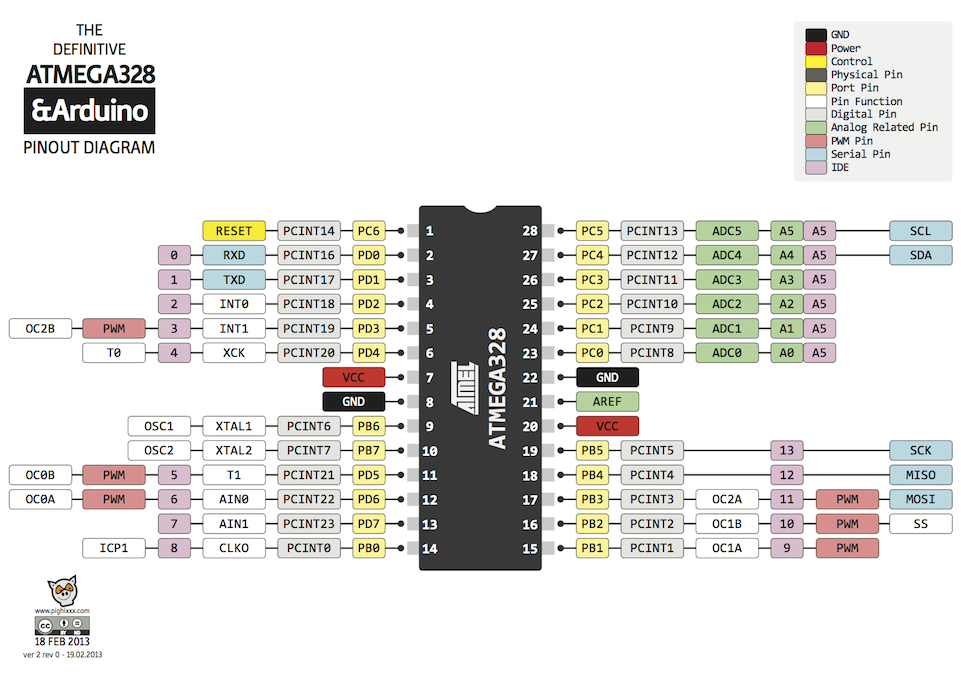
\includegraphics[width=1\linewidth]{Figures/a328diagram.png}
    \caption{Диаграмма портов ATmega328 для Arduino}
    \label{fig:a328diagram}
\end{figure}

В результате получаем значительный прирост скорости:

\begin{longtable}[c]{|c|c|}
    \caption{Результат работы напрямую с портами}
    \label{PortsResult}\\
    \hline
    \textbf{Количество, шт} & \textbf{Результат, мкс}\\
    \hline
    \endfirsthead
    \hline
    \textbf{Количество, шт} & \textbf{Результат, мкс}\\
    \hline
    \endhead
        1 & 6916\\
        \hline
        235 & 6940\\
        \hline
        328 & 6944\\
        \hline
        821 & 6948\\
        \hline
\end{longtable}

\begin{figure}[ht]
    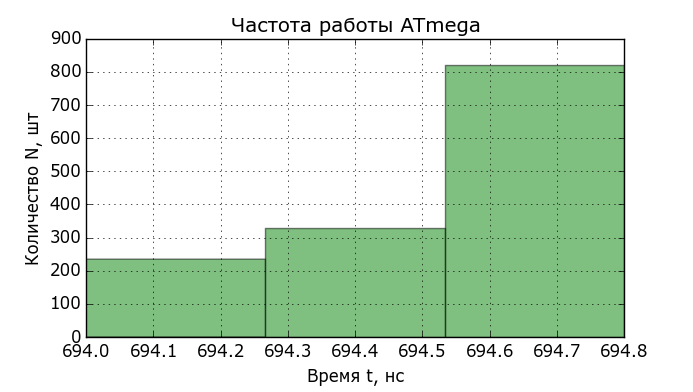
\includegraphics[width=.8\linewidth]{Figures/athist.png}
    \caption{Гистограмма измерений частоты ATmega}
    \label{fig:athist}
\end{figure}

То есть за счёт использования более низкого уровня взаимодействия с железом, мы добились увеличения скорости в $\frac{145928}{6948} = 21$ раз!

В итоге, максимальная скорость сигнала равна

\begin{equation}
    \label{eq:freq2}
    f = \frac{n}{t} = \frac{10000}{6948 \cdot 10^{-6}} = 1439263~\textrm{Гц} = 1.44~\textrm{МГц}
\end{equation}


        \subsection{Максимальная скорость бибиотеки VirtualWire}
        \label{sec:virtualwirefreq}
        Библиотека VirtualWire представляет собой высокоуровневую надстройку над Arduino для удобной передачи сообщений на расстоянии путём радиосигнала. Так как сама библиотека сложна и содержит множество задержек, замерим непосредственно минимальное время отправки сигнала --- максимальную частоту работы VirtualWire.

В целях эксперимента напишем программу, которая будет посылать один ASCII-символ данных типа \textbf{char}, занимающий ровно 1 байт (8 бит). Для обеспечения максимальной скорости, не будем ждать пока сообщение будет полностью отправлено, а будем сразу посылать следующее (если это позволит нам сделать сама \textit{VirtualWire}):

\begin{minted}[gobble=4,fontsize=\footnotesize]{c}
    #include <VirtualWire.h>
    unsigned long initial = 0; //0 - 4,294,967,295
    unsigned long final = 0;
    int i; //-32,768 - 32,767

    int TX_PIN = 1;

    const char *msg = "1";
    uint8_t buf[VW_MAX_MESSAGE_LEN];
    uint8_t buflen = VW_MAX_MESSAGE_LEN;

    void setup(){
        Serial.begin(9600);

        vw_set_tx_pin(TX_PIN);
        vw_set_ppt_inverted(true);
        vw_setup(2000);
    }

    void loop(){
        initial = micros();
        for (i = 0; i < 10; i++){
            vw_send((uint8_t *)msg, strlen(msg));
            //vw_wait_tx(); //Wait for message gone
        }
        final = micros();
        Serial.println(final - initial);
        while (final > 1E7); //Stop after 10 seconds
    }
\end{minted}

На выходе получается:

\begin{longtable}[c]{|c|c|}
    \caption{Результат использования VirtualWire}
    \label{VirtualWireResult}\\
    \hline
    \textbf{Количество, шт} & \textbf{Результат, мкс}\\
    \hline
    \endfirsthead
    \hline
    \textbf{Количество, шт} & \textbf{Результат, мкс}\\
    \hline
    \endhead
        7 & 480536\\
        \hline
        6 & 480540\\
        \hline
        7 & 480544\\
        \hline
\end{longtable}

Можно заметить, что в этом испытании было проведено лишь 10 итераций, что в итоге даёт нам частоту, не превышающую:

\begin{equation}
    \label{eq:freq3}
    f = \frac{n}{t} = \frac{10}{480540 \cdot 10^{-6}} = 20~\textrm{Гц}
\end{equation}

По-сути, VirtualWire способна передавать данные с максимальными скоростями вплоть до скоростей датчиков (9600 Кбит/с для FS1000A), однако это скорость передачи цельного блока данных. При передачи одного байта задержки складываются из-за больших битовых затрат на инициализацию драйвера передачи данных, формирование <<шапки>> пакета и проверки надежности доставки данных.

Таким образом, для наших целей библиотека VirtualWire не подходит.


    \section{Характеристика радиомодуля FS1000A + datasheet}
    \label{sec:fs1000a}
    Радиопередающий модуль FS1000A представляет собой низкобюджетное устройство передачи радиосообщений (рисунок~\ref{fig:fs1000a}). Спецификация FS1000A представлена ниже~\cite{fs1000a:specs}:

\begin{figure}[ht]
    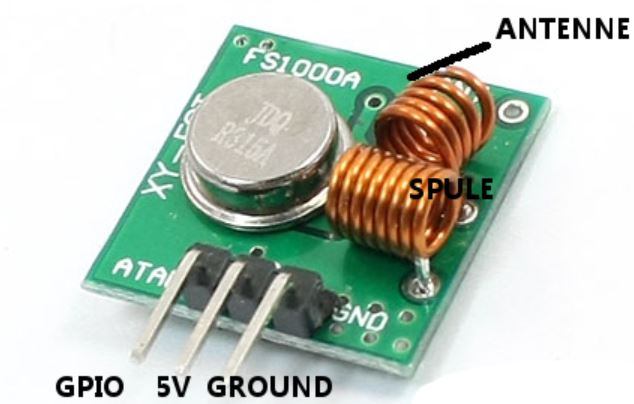
\includegraphics[width=.3\linewidth]{Figures/fs1000a.jpg}
    \caption{Радиопередатчик FS1000A}
    \label{fig:fs1000a}
\end{figure}

\begin{longtable}[c]{|c|c|}
    \caption{Спецификация модуля FS1000A}
    \label{tab:specs}\\
    \hline
    \textbf{Параметр} & \textbf{Значение}\\
    \hline
    \endfirsthead
    \hline
    \textbf{Параметр} & \textbf{Значение}\\
    \hline
    \endhead
        Входное напряжение & 2.5 -- 12 В\\
        \hline
        Тип модуляции & Амплитудная\\
        \hline
        Максимальная скорость передачи данных & 9.6 Кбит/с\\
        \hline
\end{longtable}

Скорость передачи данных в данном случае говорит, что за одну секунду можно передать блок данных размером в $\frac{9.6}{8} = 1.2$ Кб, или 9600 бит. Другими словами, если отправлять пачку длиной в 1 бит как полноценное сообщение с передатчика на приёмник, максимально доступной частотой для нас будет 9.6 КГц. Однако для надёжной передачи сообщения необходимо \textbf{как минимум} 3 бита: синхронизирующий бит, бит данных и ещё один бит данных, представляющий собой инверсию данных для подтверждения подлинности. Естественно, чем больше битов в синхронизирующем сообщении и в самом сообщении, тем надёжнее будет посылка.

Если взглянуть в справочник по передачи данных на физическом уровне (через UART), можно также заметить, что стандартное время передачи одного символа (12 бит) на скорости 9600 бит/с не превышает 1.25 мсек (рисунок~\ref{fig:mits})~\cite{mits:fx}:

\begin{figure}[ht]
    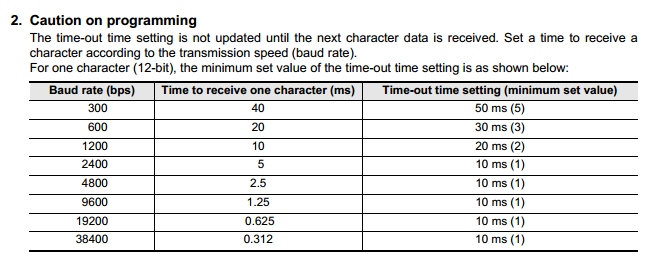
\includegraphics[width=1\linewidth]{Figures/mits.png}
    \caption{Скорость передачи данных (PLC Data Communication Manual)}
    \label{fig:mits}
\end{figure}


    %\section{Разработка программной модели}

        %\subsection{Собственная библиотека передачи данных}
        %\subsection{Программа-передатчик}
        %\subsection{Программа-ретранслятор}

    %\section{Разработка физической модели}

        %\subsection{Arduino-based setup (fritzing)}
        %\subsection{ATmega-based setup}
        %\subsection{Circuitry}
        %\subsection{PCB wiring diagram}

    %\section{Расчёт погрешностей и ошибок оборудования}

        %SPECIFIC MAIN part

    \section*{Заключение}
    \addcontentsline{toc}{section}{Заключение}
    В ходе выполнения дипломного проекта был исследован процесс передачи информации по радиоканалу и определение расстояния методом Time of Flight. Были проанализированы погрешности и задержки, возникающие как в аппаратной, так и в программной части. Были выявлены основные недостатки и предложены пути увеличения точности и скорости работы. Был сконструирован абстрактный модуль определения расстояния методом Time of Flight (аппаратная и программная часть), а также предложено оптимальное оборудование для достижения наилучших результатов.

Исследуемая система обеспечивает определение расстояния между узлами технологического процесса для дальнейшего использования этих данных в диспетчерских (SCADA) системах.


    \bibliography{web,books}

    \section*{Приложение А --- Arduino UNO Reference Design}
    \addcontentsline{toc}{section}{Приложение А --- Datasheet Arduino}
    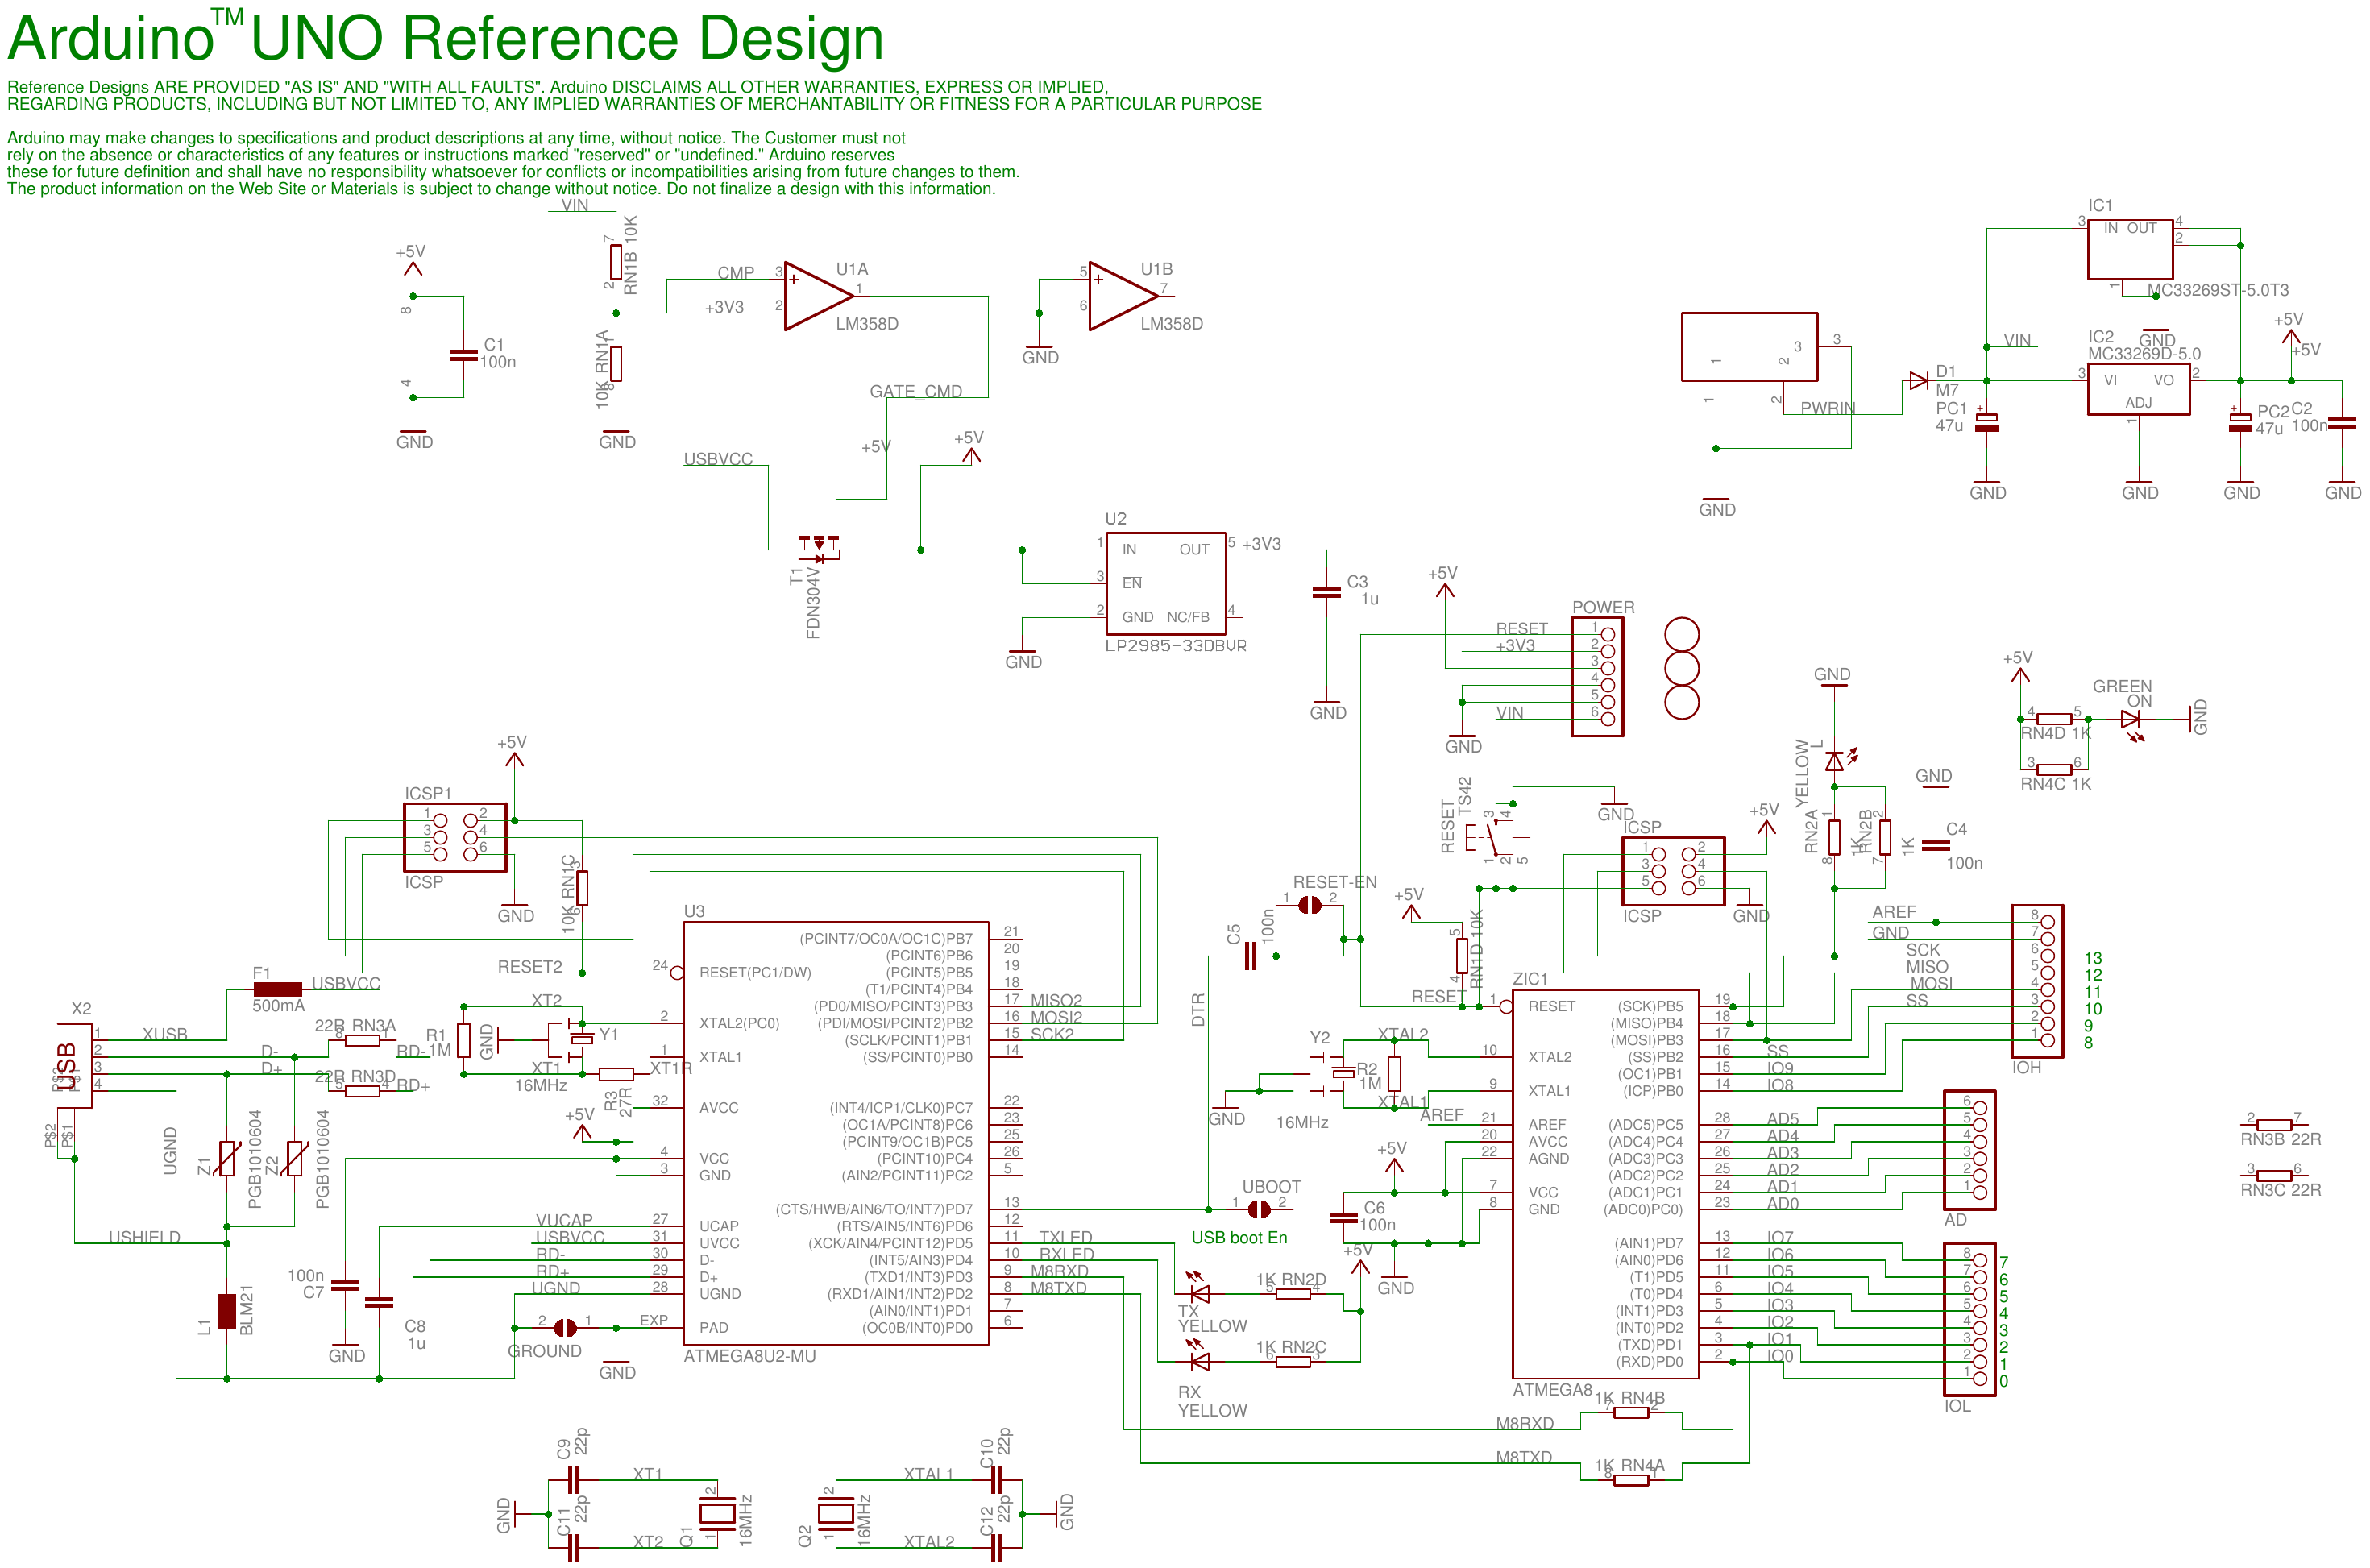
\includegraphics[angle=90,width=.9\linewidth]{Figures/arduinodatasheet.png}
   
\end{minted}
